\chapter{Экспериментальный раздел}

\section{Цель эксперимента}

Целью эксперимента является проверка правильности выполнения поставленной задачи, оценка эффективности при многопоточной реализации алгоритма обратной трассировки лучей.

\section{Апробация}

На рисунках \ref{shadows_1} -- \ref{shadows_2} представлена одна и та же сцена с различных ракурсов. Перемещение камеры и отображение теней не исказилось.

\begin{figure}[H]
	\begin{center}
		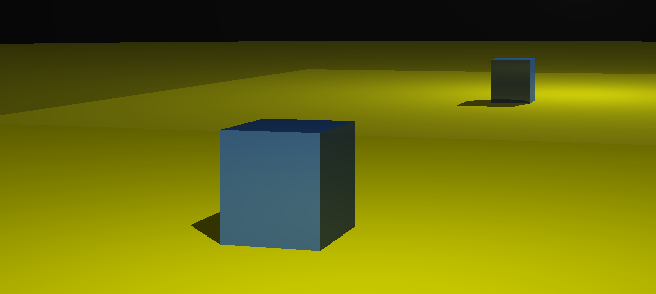
\includegraphics[scale=0.53]{assets/shadows_1.png}
	\end{center}
	\caption{Проверка камеры и теней - 1}
	\label{shadows_1}
\end{figure}

\begin{figure}[H]
	\begin{center}
		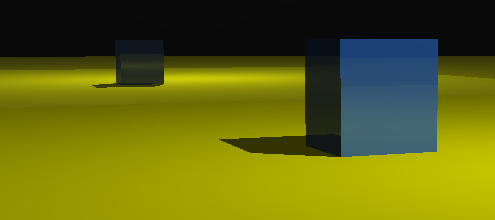
\includegraphics[scale=0.7]{assets/shadows_2.png}
	\end{center}
	\caption{Проверка камеры и теней - 2}
	\label{shadows_2}
\end{figure}

На рисунках \ref{light_1} -- \ref{light_2} представлена одна и та же сцена при разных положениях источника света. Изменение его положения работает корректно.

\begin{figure}[H]
	\begin{center}
		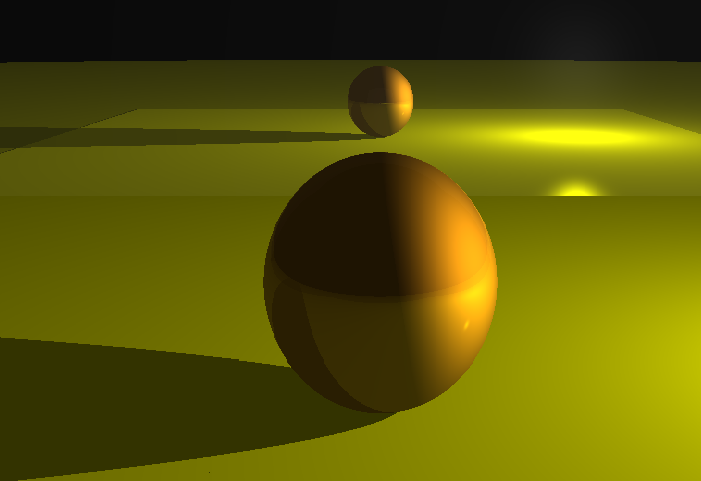
\includegraphics[scale=0.53]{assets/light_1.png}
	\end{center}
	\caption{Проверка освещения - 1}
	\label{light_1}
\end{figure}

\begin{figure}[H]
	\begin{center}
		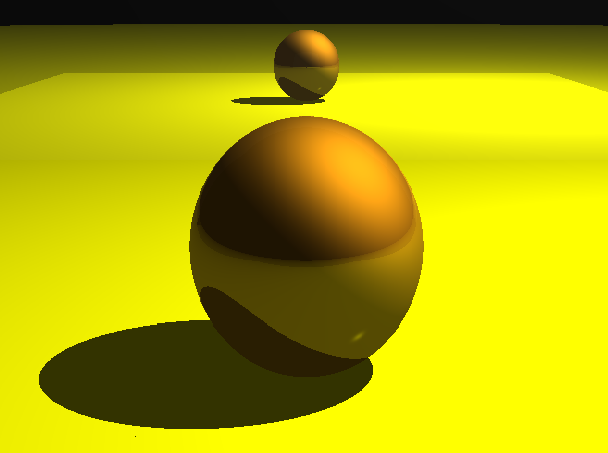
\includegraphics[scale=0.6]{assets/light_2.png}
	\end{center}
	\caption{Проверка освещения - 2}
	\label{light_2}
\end{figure}

На рисунках \ref{diffuse_1} -- \ref{diffuse_2} представлена сцена с разными значениями диффузной составляющей покрытия зеркала. На первом рисунке она равна 0, на втором -- 0.3. В случае ненулевой диффузной составляющей отражение становится нечетким, ребра перестают быть четкими в отражении, сильно проявляется гранулярность.

\begin{figure}[H]
	\begin{center}
		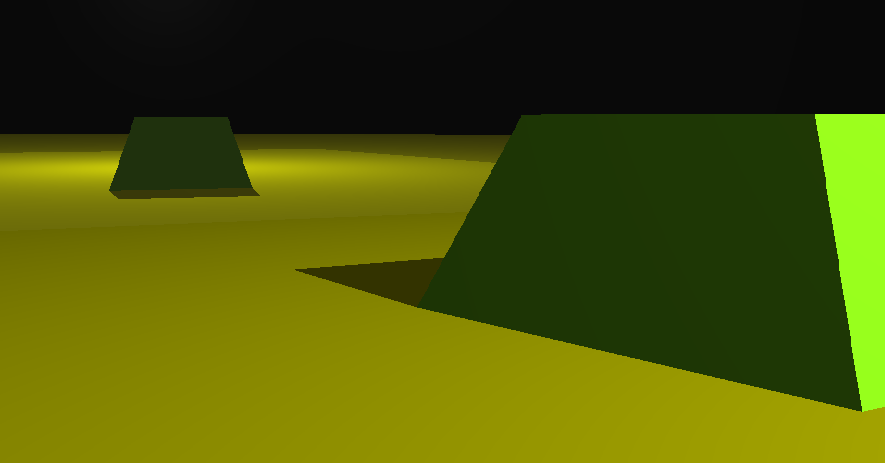
\includegraphics[scale=0.41]{assets/diffuse_1.png}
	\end{center}
	\caption{Проверка диффузной составляющей зеркала - 1}
	\label{diffuse_1}
\end{figure}

\begin{figure}[H]
	\begin{center}
		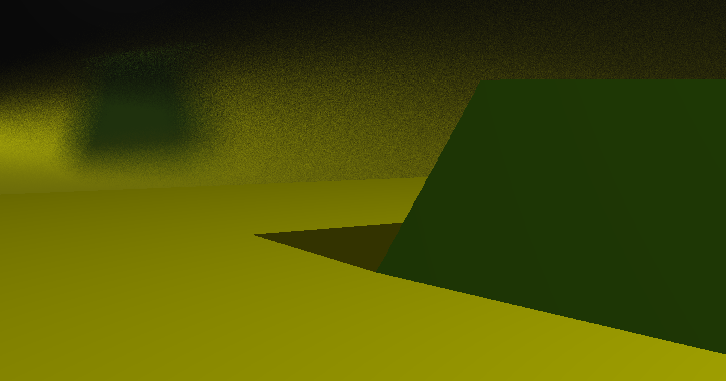
\includegraphics[scale=0.5]{assets/diffuse_2.png}
	\end{center}
	\caption{Проверка диффузной составляющей зеркала - 2}
	\label{diffuse_2}
\end{figure}

\section{Описание эксперимента}

Была замерена скорость построения изображения с двумя сферами, одна из которых имеет коэффициент отражаемости 0.7 и степень шершавости 0.05, другая с нулевым коэффициентом отражаемости, призмой и усеченной пирамидой, обе из них со значением 0.2 зеркальности, а также куб с коэффициентом отражаемости 0.4 и степенью шершавости 0.03. Для реализации многопоточной обработки были использованы средства стандартной библиотеки C++ std::thread \cite{std_thread}.

Замеры проводились на системе со следующими характеристиками:
\begin{itemize}
	\item операционная система Ubuntu 20.04.3 LTS \cite{ubuntu};
	\item память 16 Гб;
	\item процессор Intel Core i5-1135G7 11th Gen, 2.40 Гц \cite{intel}.
\end{itemize}

На рисунке \ref{graphic} представлен график зависимости времени выполнения обратной трассировки лучей при соответствующем количестве используемых потоков.

\begin{figure}[H]
	\captionsetup{singlelinecheck = false, justification=centering}
	\centering
	\begin{tikzpicture}
		\begin{axis}[
			xlabel={количество потоков},
			ylabel={время, c},
			width=0.95\textwidth,
			height=0.3\textheight,
			xmin=0, xmax=18,
			legend pos=north west,
			xmajorgrids=true,
			grid style=dashed,
			]
			\addplot[
			color=blue,
			mark=asterisk
			]
			table [x=N, y=time]{
				N time
				1 41.9
				2 36.8
				4 25.4
				6 21.0
				8 19.6
				10 18.9
				12 19.0
				14 19.4
				16 19.9
			};
		\end{axis}
	\end{tikzpicture}
	\caption{Временная зависимость построения от количества используемых потоков}
	\label{graphic}
\end{figure}

Лучшее время достигается при распределении выполнения отрисовки на 10 потоках, производительность относительно однопоточной реализации выросла на 55\%. Дальнейшее увеличение числа потоков приводит к слишком частой смене контекста, что замедляет обработку сцены.

\section{Выводи из раздела}

В данном раздела была проведена проверка на корректность выполнения функций изменений объектов сцены, таких как камера, источник освещения и плоское зеркало. Также было установлено оптимальное число используемых потоков для реализации алгоритма обратной трассировки лучей.